% CS 6043 term-paper report: 10 pages of body, 1 column, 1-inch margins, 12 pt, single spaced.
% References start on a new page after the 10 pages.
\documentclass[12pt,letterpaper]{article}

\usepackage[T1]{fontenc}
\usepackage[utf8]{inputenc}
\usepackage{newtxtext,newtxmath}
\usepackage[margin=1in]{geometry}
\usepackage{microtype}
\usepackage{amsmath}
\usepackage{graphicx}
\usepackage{booktabs,tabularx,array}
\usepackage[table]{xcolor}
\usepackage{enumitem}
\usepackage{caption}
\usepackage{xspace}
\usepackage{tikz}
\usetikzlibrary{arrows.meta,positioning}
\usepackage[numbers,sort&compress]{natbib}
\usepackage[hidelinks]{hyperref}
\usepackage[nameinlink,capitalise]{cleveref}

\definecolor{accent}{HTML}{1D4ED8}
\definecolor{muted}{HTML}{525252}
\hypersetup{colorlinks=true,linkcolor=accent,citecolor=accent,urlcolor=accent}
\setlist{itemsep=1pt,topsep=3pt}
\captionsetup{font=small,labelfont=bf}
\newcolumntype{L}[1]{>{\raggedright\arraybackslash}p{#1}}
\newcolumntype{Y}{>{\raggedright\arraybackslash}X}
\newcommand{\RQ}[1]{\textbf{RQ#1}}
\makeatletter
\renewcommand\paragraph{\@startsection{paragraph}{4}{\z@}{1.2ex \@plus .4ex \@minus .2ex}{-0.8em}{\normalfont\normalsize\bfseries}}
% \bstctlcite comes from IEEEtran.cls; defined here so IEEEtranN.bst can read its control entry
\def\bstctlcite{\@ifnextchar[{\@bstctlcite}{\@bstctlcite[@auxout]}}
\def\@bstctlcite[#1]#2{\@bsphack\@for\@citeb:=#2\do{\edef\@citeb{\expandafter\@firstofone\@citeb}\if@filesw\immediate\write\csname #1\endcsname{\string\citation{\@citeb}}\fi}\@esphack}
\makeatother
\setlength{\textfloatsep}{12pt plus 2pt minus 4pt}

% numbers generated by review/scripts/select_top50.py and case_study/plot_case_study.py (do not edit by hand)
% generated by review/scripts/select_top50.py (do not edit by hand)
\newcommand{\nAllIdentified}{2{,}459\xspace}
\newcommand{\nAllIdentifiedDB}{567\xspace}
\newcommand{\nAllIdentifiedOther}{1{,}892\xspace}
\newcommand{\nAllReports}{396\xspace}
\newcommand{\nFlowAfterDup}{2{,}396\xspace}
\newcommand{\nFlowAssessed}{427\xspace}
\newcommand{\nFlowBackward}{151\xspace}
\newcommand{\nFlowDup}{63\xspace}
\newcommand{\nFlowExFT}{31\xspace}
\newcommand{\nFlowExTA}{1{,}954\xspace}
\newcommand{\nFlowForward}{275\xspace}
\newcommand{\nFlowForwardFound}{446\xspace}
\newcommand{\nFlowKnown}{6\xspace}
\newcommand{\nFlowNotRet}{15\xspace}
\newcommand{\nFlowSought}{442\xspace}
\newcommand{\nFlowUpdate}{1{,}460\xspace}
\newcommand{\nRestAB}{249\xspace}
\newcommand{\nRestCode}{18\xspace}
\newcommand{\nRestDesign}{282\xspace}
\newcommand{\nRestEmp}{310\xspace}
\newcommand{\nRestEmu}{34\xspace}
\newcommand{\nRestFT}{62\xspace}
\newcommand{\nRestFair}{51\xspace}
\newcommand{\nRestFormal}{2\xspace}
\newcommand{\nRestGen}{28\xspace}
\newcommand{\nRestHybrid}{78\xspace}
\newcommand{\nRestKN}{1\xspace}
\newcommand{\nRestKnown}{204\xspace}
\newcommand{\nRestMedian}{1\xspace}
\newcommand{\nRestN}{312\xspace}
\newcommand{\nRestNR}{106\xspace}
\newcommand{\nRestPctCode}{6\xspace}
\newcommand{\nRestPctFT}{20\xspace}
\newcommand{\nRestPctFair}{18\xspace}
\newcommand{\nRestPctGen}{10\xspace}
\newcommand{\nRestPctHybrid}{28\xspace}
\newcommand{\nRestPctRealKnown}{19\xspace}
\newcommand{\nRestPctSimKnown}{64\xspace}
\newcommand{\nRestPctSince}{70\xspace}
\newcommand{\nRestReal}{39\xspace}
\newcommand{\nRestSim}{131\xspace}
\newcommand{\nRestSince}{218\xspace}
\newcommand{\nTopAB}{29\xspace}
\newcommand{\nTopActBitrate}{6\xspace}
\newcommand{\nTopActCwnd}{13\xspace}
\newcommand{\nTopActNet}{4\xspace}
\newcommand{\nTopActParam}{8\xspace}
\newcommand{\nTopActRate}{12\xspace}
\newcommand{\nTopCiteMedian}{52.5\xspace}
\newcommand{\nTopCode}{7\xspace}
\newcommand{\nTopContribAnalysis}{3\xspace}
\newcommand{\nTopContribFramework}{4\xspace}
\newcommand{\nTopCtrlSender}{33\xspace}
\newcommand{\nTopCut}{27\xspace}
\newcommand{\nTopDeploy}{5\xspace}
\newcommand{\nTopDesign}{43\xspace}
\newcommand{\nTopEmp}{48\xspace}
\newcommand{\nTopEmu}{11\xspace}
\newcommand{\nTopFT}{19\xspace}
\newcommand{\nTopFair}{12\xspace}
\newcommand{\nTopFormal}{2\xspace}
\newcommand{\nTopFour}{6\xspace}
\newcommand{\nTopGDataCenter}{3\xspace}
\newcommand{\nTopGInternetGeneric}{36\xspace}
\newcommand{\nTopGIotAdHocSensor}{4\xspace}
\newcommand{\nTopGSatelliteSpace}{1\xspace}
\newcommand{\nTopGWirelessCellular}{6\xspace}
\newcommand{\nTopGen}{7\xspace}
\newcommand{\nTopHybrid}{15\xspace}
\newcommand{\nTopKN}{2\xspace}
\newcommand{\nTopKnown}{42\xspace}
\newcommand{\nTopMax}{497\xspace}
\newcommand{\nTopMedian}{2\xspace}
\newcommand{\nTopN}{50\xspace}
\newcommand{\nTopNR}{6\xspace}
\newcommand{\nTopNoCount}{9\xspace}
\newcommand{\nTopPctCode}{16\xspace}
\newcommand{\nTopPctFT}{38\xspace}
\newcommand{\nTopPctFair}{28\xspace}
\newcommand{\nTopPctGen}{16\xspace}
\newcommand{\nTopPctHybrid}{35\xspace}
\newcommand{\nTopPctRealKnown}{43\xspace}
\newcommand{\nTopPctSimKnown}{31\xspace}
\newcommand{\nTopPctSince}{8\xspace}
\newcommand{\nTopReal}{18\xspace}
\newcommand{\nTopRest}{312\xspace}
\newcommand{\nTopRestOfSettings}{14\xspace}
\newcommand{\nTopSim}{13\xspace}
\newcommand{\nTopSince}{4\xspace}
\newcommand{\nTopStudies}{362\xspace}
\newcommand{\nTopTied}{4\xspace}

% generated by case_study/plot_case_study.py -- do not edit
\newcommand{\nCsNarrowRefUtil}{96\xspace}
\newcommand{\nCsNarrowRefQ}{0.03\xspace}
\newcommand{\nCsNarrowWorstUtil}{29\xspace}
\newcommand{\nCsNarrowJitterTenUtil}{29\xspace}
\newcommand{\nCsNarrowBwTwoHundredUtil}{63\xspace}
\newcommand{\nCsNarrowLossFiveUtil}{94\xspace}
\newcommand{\nCsNarrowVarQ}{0.71\xspace}
\newcommand{\nCsBroadRefUtil}{94\xspace}
\newcommand{\nCsBroadRefQ}{0.09\xspace}
\newcommand{\nCsBroadWorstUtil}{49\xspace}
\newcommand{\nCsBroadJitterTenUtil}{69\xspace}
\newcommand{\nCsBroadBwTwoHundredUtil}{69\xspace}
\newcommand{\nCsBroadLossFiveUtil}{93\xspace}
\newcommand{\nCsBroadVarQ}{0.48\xspace}
\newcommand{\nCsAimdRefUtil}{99\xspace}
\newcommand{\nCsAimdRefQ}{0.72\xspace}
\newcommand{\nCsAimdWorstUtil}{44\xspace}
\newcommand{\nCsAimdJitterTenUtil}{99\xspace}
\newcommand{\nCsAimdBwTwoHundredUtil}{87\xspace}
\newcommand{\nCsAimdLossFiveUtil}{44\xspace}
\newcommand{\nCsAimdVarQ}{1.78\xspace}
\newcommand{\nCsBbrRefUtil}{100\xspace}
\newcommand{\nCsBbrRefQ}{0.09\xspace}
\newcommand{\nCsBbrWorstUtil}{92\xspace}
\newcommand{\nCsBbrJitterTenUtil}{100\xspace}
\newcommand{\nCsBbrBwTwoHundredUtil}{95\xspace}
\newcommand{\nCsBbrLossFiveUtil}{95\xspace}
\newcommand{\nCsBbrVarQ}{1.76\xspace}
\newcommand{\nCsSeeds}{4\xspace}
\newcommand{\nCsSteps}{5\xspace}
\newcommand{\nCsTrainMinutes}{9\xspace}
\newcommand{\nCsCollapsed}{1\xspace}
\newcommand{\nCsCollapsedUtil}{3\xspace}

\xspaceaddexceptions{\%}

\title{\vspace{-1.5cm}\textbf{Reinforcement Learning for Congestion Control:\\ A Review of the \nTopN Most-Cited Studies}}
\author{Gaurab Baral \and Nityashree Vangala}
\date{CS 6043: Computer Networking, Fall 2026}

\begin{document}
\bstctlcite{IEEEexample:BSTcontrol}
\maketitle
\vspace{-0.6cm}

% ======================================================================
\section{Introduction}
\label{sec:intro}

Every time we load a web page or join a video call, a congestion control (CC) algorithm on the sending machine decides how fast to send. If it sends too slowly, the link sits idle. If it sends too fast, packets pile up in router buffers, delay grows, and eventually packets are dropped. The first widely used answer came from Jacobson after the Internet's congestion collapses of 1986: start slowly, grow the sending window a little each round trip, and cut it in half when a packet is lost~\cite{jacobson1988congestion}. Versions of that idea still run on most computers today.

The networks those rules were written for have changed a lot. Data now crosses gigabit fiber, crowded Wi-Fi, cellular links whose capacity jumps around every few milliseconds, satellite paths, and data-center fabrics where a round trip takes tens of microseconds. Researchers have answered with a long line of hand-designed algorithms: CUBIC~\cite{ha2008cubic} and BBR~\cite{cardwell2016bbr} for the Internet, DCTCP~\cite{alizadeh2010dctcp} for data centers, and many more. Each encodes a designer's guess about the network and works best in the setting it was tuned for.

Reinforcement learning (RL) offers another way to build a controller. Instead of writing the rules by hand, we let an agent try sending rates, watch what happens, and learn from a reward that scores throughput, delay and loss. Remy~\cite{winstein2013remy} and PCC~\cite{dong2015pcc} showed that machine-generated or online-learned controllers could beat hand-tuned ones, and Aurora~\cite{jay2019aurora} turned Internet congestion control into a deep RL problem in 2019. After that the number of papers grew quickly. We picked this topic because the results we kept running into looked very good on paper, yet almost nobody seemed to run these controllers in practice, and we wanted to know why.

We organized the review around three research questions:
\begin{description}[leftmargin=1.1cm,labelwidth=0.9cm]
  \item[\RQ{1}] \textbf{Design.} What do RL congestion controllers observe, what do they change, and what reward do they learn from?
  \item[\RQ{2}] \textbf{Testing.} How are they trained and tested, and do they still work on networks they did not see during training?
  \item[\RQ{3}] \textbf{Deployment.} What stops operators from using them, and what research could fix that?
\end{description}

\noindent Our search followed the PRISMA~2020 guideline for systematic reviews~\cite{page2021prisma} and found \nTopStudies eligible studies published between 2016 and 2026. Reading all of them in depth was not possible in one semester, so this report reviews the \nTopN with the most citations. We also ran a small experiment of our own: we trained two PPO controllers on different sets of simulated links and tested both on conditions they had not seen, to check one of the patterns we found in the literature.

% ======================================================================
\section{Detailed Description}
\label{sec:description}

\subsection{How congestion control works}

A good congestion controller has several jobs at once. It should fill the bottleneck link, avoid building long queues or losing packets, share the link fairly with other flows, react quickly when conditions change, and get along with the algorithms already running on the Internet. Ware et al.\ argue that a new algorithm should be judged by how much \emph{harm} it does to existing traffic~\cite{ware2019beyond}, since a scheme that starves CUBIC flows will never be allowed onto a shared network.

A sender cannot see inside the network, so it has to guess what is happening from the signals it gets back: packet loss, the round-trip time (RTT) and how it is trending, the rate at which data is being delivered, and Explicit Congestion Notification (ECN) marks that routers can set instead of dropping packets. It acts through one of two knobs. The \emph{congestion window} (cwnd) limits how much unacknowledged data can be in flight, and the \emph{pacing rate} spaces packets out in time.

Classic algorithms differ in which signal they trust. Reno grows the window by one packet per RTT and halves it on loss~\cite{rfc5681}. CUBIC, the Linux default, grows the window as a cubic function of the time since the last loss, which lets it recover faster on long, fast paths~\cite{ha2008cubic}. Vegas backs off as soon as the RTT rises above its minimum~\cite{brakmo1995vegas}, which keeps queues short but loses out to loss-based flows. BBR builds a model instead: it estimates the bottleneck bandwidth and the minimum RTT and paces at the estimated bandwidth~\cite{cardwell2016bbr}. Routers can help too. Active queue management schemes such as RED~\cite{floyd1993red} and CoDel~\cite{nichols2012codel} drop or mark packets before the buffer fills, and in data centers DCTCP cuts its window in proportion to the fraction of ECN-marked packets~\cite{alizadeh2010dctcp}. DCTCP's marking threshold is usually tuned by hand, which is one place RL has been tried.

\subsection{Reinforcement learning in brief}

RL treats a problem as a loop between an agent and an environment, written as a Markov decision process. At each step $t$ the agent observes a state $s_t$, picks an action $a_t$ using its policy $\pi$, receives a reward $r_t$, and the environment moves to a new state $s_{t+1}$. The agent's goal is a policy that maximizes the expected discounted return $\mathbb{E}[\sum_t \gamma^t r_t]$, where $\gamma<1$ makes near-term rewards count more than distant ones~\cite{sutton2018reinforcement}. A sender only sees its own feedback and never the full state of the network, so congestion control is really a partially observable problem. Most designs deal with this by giving the agent a short history of recent measurements.

The studies we reviewed use several families of RL methods. \emph{Value-based} methods learn how good each action is in each state; Q-learning does this with a table and the Deep Q-Network (DQN) with a neural network~\cite{mnih2015human}. \emph{Policy-gradient} methods such as PPO~\cite{schulman2017ppo} adjust the policy directly and handle continuous actions like ``multiply the rate by 1.03'' easily. \emph{Off-policy actor-critic} methods such as TD3~\cite{fujimoto2018td3} reuse past experience stored in a replay buffer, which makes them more sample efficient. A few studies use \emph{offline RL}, which learns only from logged data without trying new actions online, \emph{imitation learning}, which copies an expert, \emph{contextual bandits}, which treat every decision as a one-step problem, or \emph{multi-agent RL}, where several agents such as competing flows learn together.

\subsection{Congestion control as an RL problem}

\Cref{fig:loop} shows the formulation that Aurora made popular~\cite{jay2019aurora}, and most later papers follow it closely. Time is split into short \emph{monitor intervals}. At the start of each interval the agent chooses an action. When the acknowledgments for that interval come back, the sender computes statistics such as throughput, average RTT and loss rate, turns them into the next state, and computes a reward.

\begin{figure}[t]
\centering
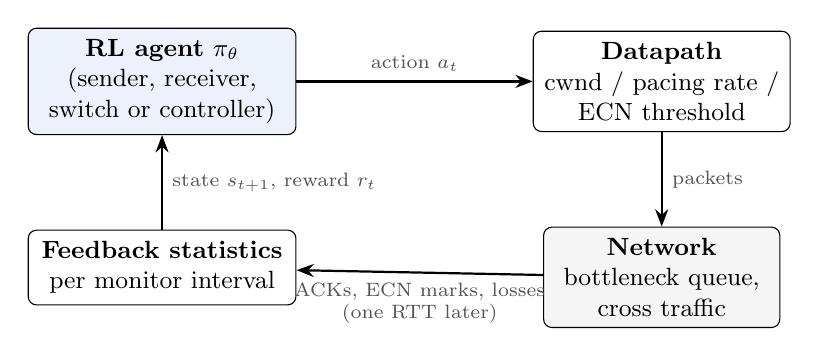
\begin{tikzpicture}[
  box/.style={draw, rounded corners=3pt, align=center, minimum height=9mm, inner sep=4pt, font=\small},
  lab/.style={font=\scriptsize, align=center, text=muted},
  >={Stealth[length=2.2mm]}]
  \node[box, fill=accent!8, minimum width=34mm] (agent) {\textbf{RL agent} $\pi_\theta$\\ (sender, receiver,\\ switch or controller)};
  \node[box, right=30mm of agent, minimum width=30mm] (dp) {\textbf{Datapath}\\ cwnd / pacing rate /\\ ECN threshold};
  \node[box, below=12mm of dp, minimum width=30mm, fill=black!4] (net) {\textbf{Network}\\ bottleneck queue,\\ cross traffic};
  \node[box, below=12mm of agent, minimum width=34mm] (stats) {\textbf{Feedback statistics}\\ per monitor interval};
  \draw[->, thick] (agent) -- node[above, lab]{action $a_t$} (dp);
  \draw[->, thick] (dp) -- node[right, lab]{packets} (net);
  \draw[->, thick] (net) -- node[below, lab]{ACKs, ECN marks, losses\\(one RTT later)} (stats);
  \draw[->, thick] (stats) -- node[right, lab]{state $s_{t+1}$, reward $r_t$} (agent);
\end{tikzpicture}
\caption{The usual RL congestion-control loop. The agent acts once per monitor interval and sees the results about one RTT later.}
\label{fig:loop}
\end{figure}

Within this loop, designers have to make five choices.
\begin{enumerate}
  \item \textbf{Where the agent runs.} Most agents run at the sender. For real-time video the agent often runs at the receiver, and in data centers it can sit in each switch or in a central controller.
  \item \textbf{What it observes.} Typical inputs are recent throughput, RTT, the RTT gradient, loss rate and the current window or rate. Aurora deliberately used ratios (latency gradient, latency ratio and sending ratio) so that the same policy could work at different link speeds.
  \item \textbf{What it changes.} The action can set the window or rate directly, tune a parameter of a classic algorithm, choose among several existing algorithms, or set something in the network such as an ECN threshold.
  \item \textbf{What it is rewarded for.} Most rewards add up throughput and subtract penalties for delay and loss.
  \item \textbf{How often it acts.} Running a neural network on every ACK is too slow at high speeds, so most designs act once per interval.
\end{enumerate}

The reward deserves a closer look, because it decides what the controller will do. Aurora's reward is $10\cdot\text{throughput} - 1000\cdot\text{latency} - 2000\cdot\text{loss}$, with throughput in packets per second, latency in seconds and loss as a fraction. To see what the weights mean, take a 10\,Mbit/s link (about 830 packets per second of 1500 bytes) with a 50\,ms RTT. A sender that fills the link earns about 8,300 from throughput and loses 50 for the base latency. If it overshoots and builds a 100\,ms queue, it loses another 100. That penalty is small next to the throughput term, so this reward will tolerate quite a bit of queueing to keep the link full. A reward with a larger delay weight would produce a more cautious controller. In other words, the weights act as the specification of the controller, and two papers with different weights are really solving different problems.

The problem has two more difficulties. An action's result arrives one RTT later, mixed with the effects of every other flow, so the agent struggles to tell which action caused what. And the controller will run on networks unlike its training ones, so behavior under that shift is the main test of its quality.

\subsection{How we chose the papers}

We searched OpenAlex, arXiv and the USENIX NSDI and ATC proceedings for 2016 to 2026 with the query \texttt{("reinforcement learning" OR "imitation learning") AND ("congestion control" OR "congestion window" OR "ECN")}. Our proposal also listed IEEE Xplore, the ACM Digital Library and Scopus, but their programmatic interfaces need institutional keys, so we used OpenAlex, which indexes most of the same venues. We added forward citation searching (papers that cite well-known studies such as Aurora and Orca), backward citation searching (the reference lists of recent studies), and a later search with wider terms such as ``Q-learning'', ``bandit'' and ``AQM''. These steps follow the advice of Kitchenham and Charters for systematic reviews in computing~\cite{kitchenham2007guidelines}.

We kept a study if an RL or imitation-learning method controls congestion in a packet network, or if the study builds a framework to train or test such controllers. We removed RL for other tasks such as routing, methods with no learning component, and other surveys. \Cref{fig:flow} shows how many records survived each step. To make the review manageable we then ranked the \nTopStudies included studies by their citation count in Semantic Scholar on 9~November~2026 and kept the top \nTopN; the fiftieth study has \nTopCut citations.

\begin{figure}[t]
\centering
\scalebox{0.62}{%
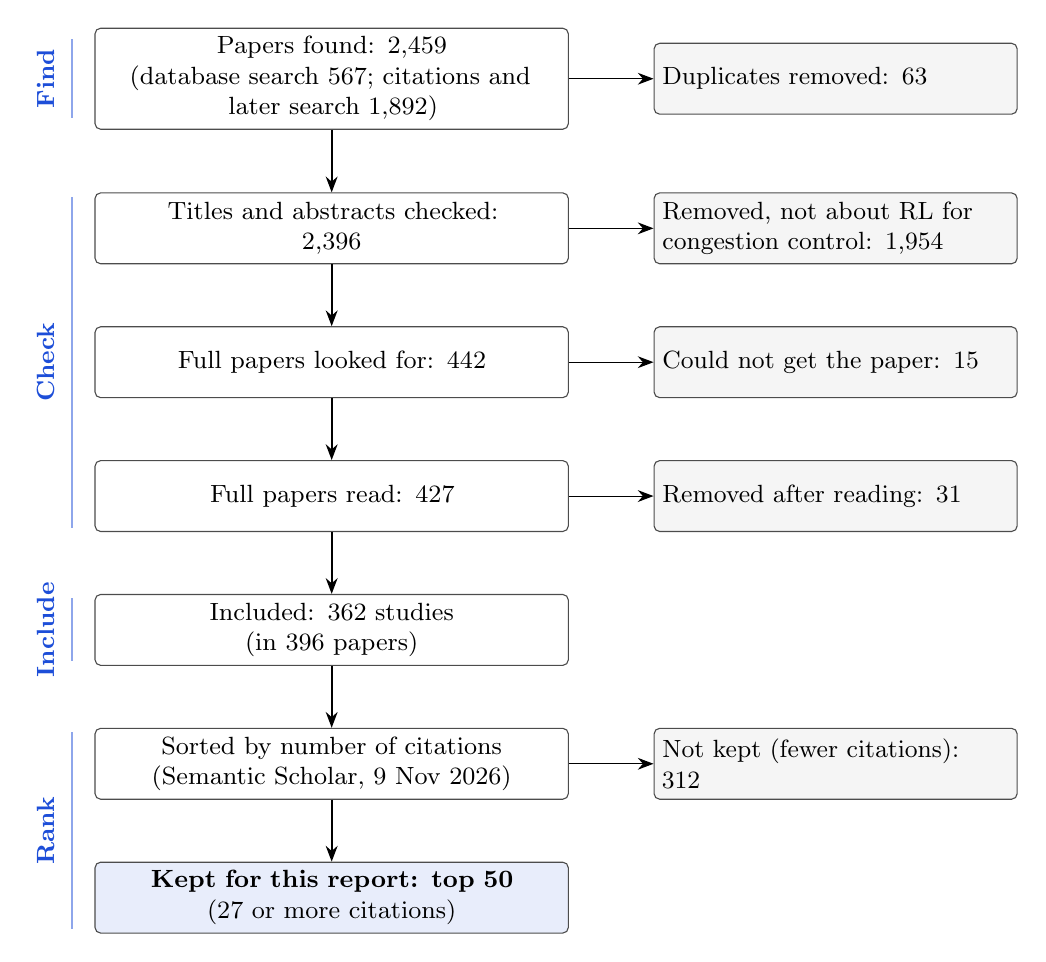
\begin{tikzpicture}[
  box/.style={draw=black!70, rounded corners=2pt, align=center, text width=58mm, minimum height=9mm, inner sep=3pt, font=\small},
  gone/.style={draw=black!70, rounded corners=2pt, align=left, text width=44mm, minimum height=9mm, inner sep=3pt, font=\small, fill=black!4},
  stage/.style={font=\small\bfseries, text=accent, rotate=90, anchor=south},
  >={Stealth[length=2mm]}]
  \node[box] (found) at (0,0) {Papers found: \nAllIdentified\\ (database search \nAllIdentifiedDB; citations and\\ later search \nAllIdentifiedOther)};
  \node[gone] (dup) at (64mm,0) {Duplicates removed: \nFlowDup};
  \node[box] (title) at (0,-19mm) {Titles and abstracts checked:\\ \nFlowAfterDup};
  \node[gone] (offtopic) at (64mm,-19mm) {Removed, not about RL for\\ congestion control: \nFlowExTA};
  \node[box] (full) at (0,-36mm) {Full papers looked for: \nFlowSought};
  \node[gone] (missing) at (64mm,-36mm) {Could not get the paper: \nFlowNotRet};
  \node[box] (read) at (0,-53mm) {Full papers read: \nFlowAssessed};
  \node[gone] (notfit) at (64mm,-53mm) {Removed after reading: \nFlowExFT};
  \node[box] (incl) at (0,-70mm) {Included: \nTopStudies studies\\ (in \nAllReports papers)};
  \node[box] (rank) at (0,-87mm) {Sorted by number of citations\\ (Semantic Scholar, 9 Nov 2026)};
  \node[gone] (rest) at (64mm,-87mm) {Not kept (fewer citations):\\ \nRestN};
  \node[box, fill=accent!10] (keep) at (0,-104mm) {\textbf{Kept for this report: top \nTopN}\\ (\nTopCut or more citations)};
  \foreach \a/\b in {found/title, title/full, full/read, read/incl, incl/rank, rank/keep} \draw[->, thick] (\a) -- (\b);
  \foreach \a/\b in {found/dup, title/offtopic, full/missing, read/notfit, rank/rest} \draw[->] (\a) -- (\b);
  \draw[accent!50, thick] (-33mm,5mm) -- (-33mm,-5mm); \node[stage] at (-34mm,0) {Find};
  \draw[accent!50, thick] (-33mm,-15mm) -- (-33mm,-57mm); \node[stage] at (-34mm,-36mm) {Check};
  \draw[accent!50, thick] (-33mm,-66mm) -- (-33mm,-74mm); \node[stage] at (-34mm,-70mm) {Include};
  \draw[accent!50, thick] (-33mm,-83mm) -- (-33mm,-108mm); \node[stage] at (-34mm,-95.5mm) {Rank};
\end{tikzpicture}}
\caption{How we chose the \nTopN studies, drawn in the style of a PRISMA~2020 flow diagram~\cite{page2021prisma}. One study can appear in several papers, such as a conference paper and its journal version.}
\label{fig:flow}
\end{figure}

For each of the \nTopN studies we recorded the network setting, where the agent runs, the RL method, the state, action and reward, and the highest level of testing it reached: \emph{simulation}, \emph{emulation} (real network software over software-imposed links), or a \emph{real network}. We also noted whether the study tested conditions outside its training range, whether it measured fairness, and whether it released code. We call a design \emph{hybrid} when a classic algorithm or safety rule stays in the control loop after deployment. Finally, each design study gets a practice score from 0 to 5, one point each for reporting the test environment, using emulation or a real network, testing generalization, measuring fairness, and releasing code.

\subsection{The designs among the \nTopN}

Of the \nTopN studies, \nTopGInternetGeneric target the wide-area Internet or a generic wired bottleneck, \nTopGWirelessCellular target wireless or cellular networks, \nTopGIotAdHocSensor target IoT or sensor networks, \nTopGDataCenter target data centers and \nTopGSatelliteSpace targets satellite links. Of the \nTopDesign studies that propose a controller, \nTopCtrlSender run the agent at the sender. \Cref{tab:landmarks} lists the designs that later papers build on most often, and the paragraphs below group the rest.

\begin{table}[t]
\centering
\caption{Landmark designs among the \nTopN. Level is the highest testing environment the study reached (Emu = emulation).}
\label{tab:landmarks}
\footnotesize
\setlength{\tabcolsep}{3pt}
\begin{tabularx}{\linewidth}{@{}L{1.7cm}L{3.1cm}YL{2.0cm}l@{}}
\toprule
Study & Action & Learning signal & Algorithm & Level \\
\midrule
Indigo~\cite{yan2018pantheon} & cwnd step every 10\,ms & imitate an oracle that knows the emulated link's ideal cwnd & imitation, LSTM & Real \\
Aurora~\cite{jay2019aurora} & rate multiplier per interval & weighted throughput, latency, loss & PPO & Emu \\
Orca~\cite{abbasloo2020orca} & scale CUBIC's cwnd by $2^{2a}$ & throughput minus loss, scaled by delay & TD3 & Real \\
MOCC~\cite{ma2022mocc} & rate & preference-weighted throughput, delay, loss & PPO & Real \\
Genet~\cite{xia2022genet} & (training method) & Aurora's reward with a curriculum & PPO & Real \\
Sage~\cite{yen2023sage} & cwnd & logged behavior of existing heuristics & offline RL & Real \\
Astraea~\cite{liao2024astraea} & rate & throughput, delay, loss, fairness & multi-agent & Real \\
Mutant~\cite{pappone2025mutant} & select a kernel CC scheme & power (throughput / delay) & LinUCB bandit & Real \\
\bottomrule
\end{tabularx}
\end{table}

\paragraph{Early Q-learning controllers.} The oldest designs in the set use Q-learning over small state spaces that the authors split into buckets by hand. QTCP approximates the Q-function with Kanerva coding and reports 59.5\% higher throughput than rule-based TCP~\cite{li2019qtcp}. These designs are simple to understand, but hand-made buckets do not scale to the wide range of link speeds and delays seen on the Internet.

\paragraph{Clean-slate deep RL.} Aurora~\cite{jay2019aurora} set the template most later work copies. It was trained with PPO on simulated links of 1.2 to 6\,Mbit/s and kept near-full utilization in emulation from 1 to 128\,Mbit/s, a range far wider than its training data. It did poorly at 1\,ms latency, though, because about 1\,ms of packet-processing noise that never appeared in training swamped its latency signal. We return to this failure in our own experiment. Indigo, released with the Pantheon testbed~\cite{yan2018pantheon}, took a different route and imitated an oracle that knew the best window for each emulated link. MVFST-RL~\cite{sivakumar2019mvfst} pointed out a problem that simulators hide: in a real network stack, packets keep flowing while the agent is still computing. It runs the policy asynchronously inside Facebook's QUIC implementation.

\paragraph{Hybrids built on classic control.} \nTopHybrid of the \nTopDesign design studies (\nTopPctHybrid\%) are hybrids. The common idea is to let a classic algorithm react to every ACK while the agent adjusts it more slowly. In Orca~\cite{abbasloo2020orca}, CUBIC runs in the Linux kernel, and once per monitoring period a TD3 agent multiplies CUBIC's window by $2^{2a}$ with $a\in[-1,1]$. Orca performed more consistently than clean-slate learned controllers and needed less computation. Spine~\cite{tian2024spine} has a slow agent that hands sub-policies to a light executor, which cuts control overhead by at least 80\%. Other designs learn \emph{which} algorithm to run. TCP-RL~\cite{nie2019tcprl} chooses the initial window and picks among 14 TCP variants on the web servers of a large search engine, and Mutant~\cite{pappone2025mutant} switches between kernel protocols using a contextual bandit.

\paragraph{Learning from logs.} Exploring online on real users' traffic is risky, so some studies learn from data that already exists. Sage~\cite{yen2023sage} trains offline on traces of existing heuristics and ends up outperforming the heuristics it learned from. Concerto~\cite{zhou2019concerto} imitated over one million logged video-call sessions.

\paragraph{Several objectives and fairness.} A fixed reward fixes one trade-off between throughput and delay. MOCC~\cite{ma2022mocc} instead feeds the policy a preference vector, so one model can serve different applications, and it adapts to a new objective 14.2 times faster than earlier work. Fairness is a separate problem: a policy trained alone tends to be greedy when copies of it share a link. Astraea~\cite{liao2024astraea} trains several flows together with a fairness term in the reward and converges to a fair share up to 8.4 times faster.

\paragraph{Other settings.} For real-time video, the controller is a bandwidth estimator that sets the encoder's bitrate. Loki~\cite{zhang2021loki} combines an RL model with a rule-based one, and OnRL~\cite{zhang2020onrl} learns online from mobile users, with a rule-based fallback that takes over when the learned policy misbehaves. In data centers, ACC~\cite{yan2021acc} runs an agent in every switch to tune ECN thresholds, and RL-CC~\cite{tessler2022rlcc} treats RDMA congestion control as a multi-agent problem. All IoT studies whose testing level we could find stop at simulation.

\subsection{How the studies are tested}

We sort testing environments by how much of the real system they include. \emph{Simulators} such as ns-3 model both the network and the hosts, and they leave out the operating system's timers, pacing and ACK batching. \emph{Emulators} such as Mininet~\cite{lantz2010mininet} and Mahimahi~\cite{netravali2015mahimahi} run real network software over links shaped in software. \emph{Testbeds and real networks}, such as Pantheon's machines spread around the world~\cite{yan2018pantheon}, cloud paths, and production traffic, put the controller on physical links. Four of the \nTopN studies are testing frameworks (Pantheon, MVFST-RL, OpenNetLab and Iroko), and two verify trained policies formally; whiRL proves some properties of Aurora and finds counterexamples to others~\cite{eliyahu2021whirl}.

% ======================================================================
\section{Results}
\label{sec:results}

\subsection{How well the studies are tested}

\Cref{tab:compare} compares the \nTopN most-cited studies with the other \nTopRest eligible studies. Of the \nTopEmp top studies with an experimental evaluation, \nTopReal reach a real network, \nTopEmu stop at emulation, \nTopSim stop at simulation and \nTopNR do not say.

\begin{table}[t]
\centering
\caption{The \nTopN most-cited studies against the other \nTopRest eligible studies. Generalization, fairness, code and hybrid are counted over design studies. Testing shares are over studies whose testing level is known.}
\label{tab:compare}
\small
\begin{tabular}{@{}lrr@{}}
\toprule
 & Top \nTopN & Other \nTopRest \\
\midrule
Design studies & \nTopDesign & \nRestDesign \\
Reach a real network & \nTopReal/\nTopKnown{} (\nTopPctRealKnown\%) & \nRestReal/\nRestKnown{} (\nRestPctRealKnown\%) \\
Simulation only & \nTopSim/\nTopKnown{} (\nTopPctSimKnown\%) & \nRestSim/\nRestKnown{} (\nRestPctSimKnown\%) \\
Test outside training range & \nTopGen{} (\nTopPctGen\%) & \nRestGen{} (\nRestPctGen\%) \\
Measure fairness & \nTopFair{} (\nTopPctFair\%) & \nRestFair{} (\nRestPctFair\%) \\
Release code & \nTopCode{} (\nTopPctCode\%) & \nRestCode{} (\nRestPctCode\%) \\
Hybrid (classic part in the loop) & \nTopHybrid{} (\nTopPctHybrid\%) & \nRestHybrid{} (\nRestPctHybrid\%) \\
First published 2023 or later & \nTopSince{} (\nTopPctSince\%) & \nRestSince{} (\nRestPctSince\%) \\
Median practice score (0--5) & \nTopMedian & \nRestMedian \\
\bottomrule
\end{tabular}
\end{table}

\paragraph{Observation 1: the most-cited studies test on real networks more often, but most still do not.} The top \nTopN reach a real network more than twice as often as the rest (\nTopPctRealKnown\% against \nRestPctRealKnown\%) and rely on simulation alone about half as often. Part of this gap comes from how much we could read: we had the full text of the top studies about twice as often, and abstracts often skip testing details.

\paragraph{Observation 2: many citations do not mean strong evidence.} The median top design scores only \nTopMedian out of 5 on our practice score. Just \nTopFour score four or more: Orca scores 5, and Aurora, Genet, MOCC, Astraea and Mutant score 4. We expected the most influential papers to set a higher bar than this.

\paragraph{Observation 3: few studies test outside their training range.} Only \nTopGen of the \nTopDesign designs test on conditions they were not trained on, and only \nTopCode release code. Without public code, later papers keep comparing against the same few open-source controllers, mostly Aurora and Orca. Deep RL results also change with random seeds~\cite{henderson2018deep}, so a result from one run is hard to trust. Where generalization does work, it comes from training on a broad, deliberately chosen set of environments or from training on the deployment's own data. Genet~\cite{xia2022genet}, for example, picks training environments where the RL policy is doing worse than rule-based baselines, and its policies beat normally trained ones on real paths.

\paragraph{Observation 4: independent tests are much less positive.} Recent independent evaluations are not in our top \nTopN, probably because they are too new to have many citations, but they matter for \RQ{2}. Giacomoni and Parisis found that public RL controllers grab bandwidth quickly and handle random loss, but cause extra loss, are unfair in almost every setup, and react slowly when conditions change~\cite{giacomoni2024rlcc}. Mazilu et al.\ report similar problems against CUBIC and BBRv3~\cite{mazilu2025learning}. Ghermezian et al.\ ran an Aurora-style controller on a real 10\,Gbit/s wide-area path, where it reached 0.5\% average utilization while CUBIC and BBR reached up to 9.9 and 9.7\,Gbit/s~\cite{ghermezian2026ppo}. Someone who read only the most-cited papers would not see any of this.

\subsection{Our experiment: what the training data does to a controller}

Observation 3 raised a question the papers could not answer: with everything else fixed, how much does the choice of training links change a controller's behavior on unseen links? We built a small simulator to find out.

\paragraph{Setup.} The simulator models one flow through one drop-tail bottleneck queue and uses Aurora's formulation. The agent acts every 20\,ms, its feedback arrives one base RTT later, and it observes the latency gradient, latency ratio and sending ratio for the last ten intervals. Each action changes the rate by at most 5\%, and the reward is utilization minus queueing delay (in RTTs) minus three times the loss rate. We trained PPO~\cite{schulman2017ppo} for \nCsSteps{} million steps with \nCsSeeds{} random seeds on each of two sets of links. The \emph{narrow} set used 1 to 5\,Mbit/s, 40 to 60\,ms RTT, buffers of 1 to 2 bandwidth-delay products (BDP), and no loss or jitter, which is close to Aurora's training range. The \emph{broad} set used 1 to 100\,Mbit/s, 10 to 200\,ms, 0.2 to 5\,BDP, up to 3\% random loss, up to 10\,ms of RTT jitter, and capacity that changes over time. We compared both against a Reno-like AIMD controller and a BBR-like controller, changing one factor at a time around a reference link of 3\,Mbit/s, 50\,ms and 1.5\,BDP. Each training run took about \nCsTrainMinutes{} minutes on one CPU core.

\begin{figure}[t]
\centering
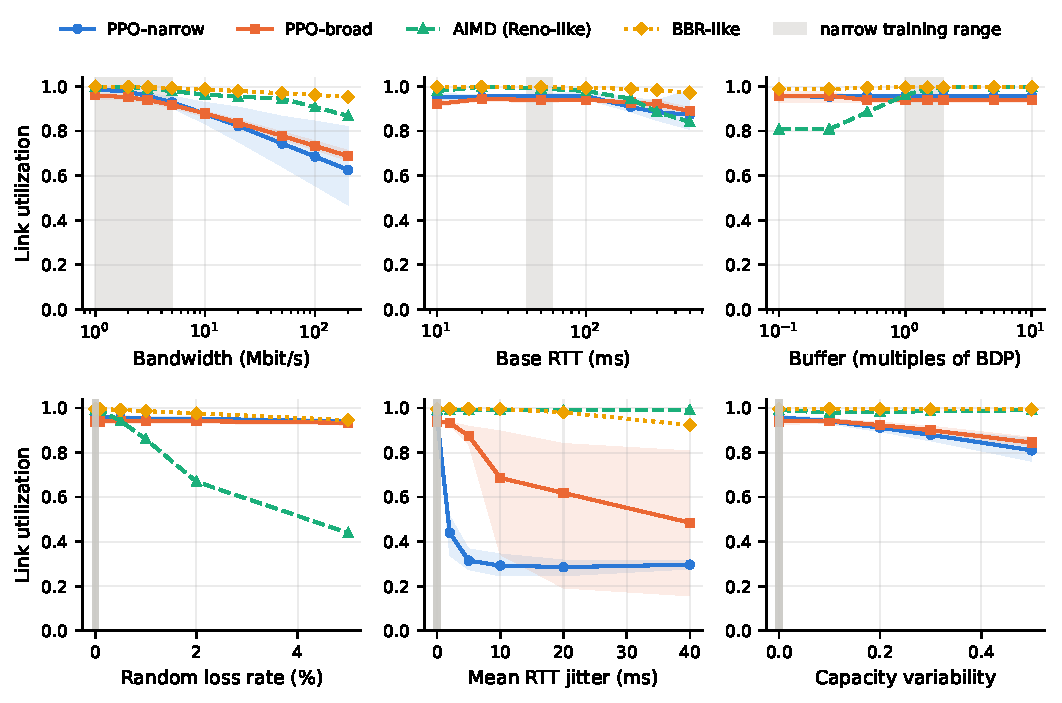
\includegraphics[width=0.8\linewidth]{../survey/figures/case_study_util.pdf}
\caption{Our experiment: link utilization when one factor is changed around the reference link. Lines are means over the training seeds that converged, and shaded bands show their spread. The gray band marks the narrow training range.}
\label{fig:case}
\end{figure}

\begin{table}[t]
\centering
\caption{Summary of our experiment, averaged over converged seeds. ``Queue'' is the mean queueing delay in multiples of the base RTT. One of the \nCsSeeds{} broad seeds failed to learn and is left out; all narrow seeds converged.}
\label{tab:case}
\small
\begin{tabular}{@{}lrrrrrr@{}}
\toprule
 & \multicolumn{2}{c}{In distribution} & \multicolumn{4}{c}{Utilization (\%) under one shifted factor} \\
\cmidrule(lr){2-3}\cmidrule(l){4-7}
Controller & Util.\ (\%) & Queue (RTT) & 200\,Mbit/s & 5\% loss & 10\,ms jitter & Worst case \\
\midrule
PPO-narrow & 96 & 0.03 & 63 & 94 & 29 & 29 (20\,ms jitter) \\
PPO-broad & 94 & 0.09 & 69 & 93 & 69 & 49 (40\,ms jitter) \\
AIMD (Reno-like) & 99 & 0.72 & 87 & 44 & 99 & 44 (5\% loss) \\
BBR-like & 100 & 0.09 & 95 & 95 & 100 & 92 (40\,ms jitter) \\
\bottomrule
\end{tabular}

\end{table}

\paragraph{What we found.} \Cref{fig:case,tab:case} show the results.
\begin{itemize}
  \item \textbf{On familiar links the learned controllers do well.} Both PPO policies reach at least \nCsBroadRefUtil\% utilization with queues of only \nCsNarrowRefQ{} to \nCsBroadRefQ{} RTT, while AIMD keeps a queue of \nCsAimdRefQ{} RTT.
  \item \textbf{A little delay noise breaks the narrow policy.} With 10\,ms of RTT jitter, which is normal on Wi-Fi and cellular links, the narrow policy's utilization drops from \nCsNarrowRefUtil\% to \nCsNarrowJitterTenUtil\%. Its latency inputs read the noise as a growing queue, so it keeps slowing down. AIMD ignores delay and BBR-like filters it, so both stay near full utilization. This is the same failure the Aurora authors saw at 1\,ms latency.
  \item \textbf{Broader training helps only inside its range.} The broad policy, which saw jitter up to 10\,ms, keeps \nCsBroadJitterTenUtil\% utilization at 10\,ms but falls to \nCsBroadWorstUtil\% at 40\,ms. It also keeps a longer queue on the reference link, and one of its four seeds never learned at all and stayed at \nCsCollapsedUtil\% utilization.
  \item \textbf{The learned controllers fail in different places than classic ones.} With 5\% random loss the PPO policies keep \nCsBroadLossFiveUtil{} to \nCsNarrowLossFiveUtil\% utilization while AIMD falls to \nCsAimdLossFiveUtil\%. A test suite built around the known weaknesses of classic algorithms would make the learned controllers look great and miss the jitter problem entirely.
  \item \textbf{Fast links expose a design limit.} At 200\,Mbit/s the PPO policies reach only \nCsNarrowBwTwoHundredUtil{} to \nCsBroadBwTwoHundredUtil\% utilization, compared with \nCsBbrBwTwoHundredUtil\% for BBR-like. Because each action can change the rate by at most 5\%, climbing two orders of magnitude takes seconds no matter what the training data looked like.
\end{itemize}

\noindent Our simulator is simple: it has one flow, a fluid queue, no competing traffic and small policies, so we do not claim these numbers for any published controller. Still, it showed that a learned controller's weak spots follow from its inputs, and a wider training set moves them instead of removing them.

\subsection{Deployment}

\Cref{tab:deployments} lists the \nTopDeploy studies among the \nTopN that report use in production or tests with real users.

\begin{table}[t]
\centering
\caption{Studies among the \nTopN that report production use or tests with real users.}
\label{tab:deployments}
\footnotesize
\setlength{\tabcolsep}{4pt}
\begin{tabularx}{\linewidth}{@{}L{1.95cm}L{1.9cm}YcL{3.45cm}@{}}
\toprule
System & Setting & Learned component & Classic in loop & Reported scale \\
\midrule
TCP-RL~\cite{nie2019tcprl} & Web search & initial window; algorithm selection & yes & search engine, over a year; 23\% shorter short flows \\
Concerto~\cite{zhou2019concerto} & Video calls & bitrate policy imitated from logs & no & production video-telephony app \\
OnRL~\cite{zhang2020onrl} & Mobile video & per-user online RL, combined model & yes & 543\,h, 151 users; 14.2\% fewer stalls \\
Loki~\cite{zhang2021loki} & Real-time video & RL fused with a rule-based model & yes & 101 million sessions; 26 to 44\% fewer stalls \\
ACC~\cite{yan2021acc} & Data center & per-switch ECN threshold & yes & 300 machines; 30\% lower flow completion time \\
\bottomrule
\end{tabularx}
\end{table}

\paragraph{Observation 5: the deployed systems share a pattern.} Every one of them is run by a company that controls the senders or the switches, so it can monitor the controller, test it on part of its traffic and roll it back. Each one optimizes a single service metric such as transfer time, video stalls or storage throughput. Four of the five keep a classic algorithm or safety rule in the loop, and the fifth, Concerto, learned only from logged sessions and never explored on live traffic. None of them is a general-purpose controller for Internet traffic.

\paragraph{What holds deployment back.} Putting the papers and our experiment together, we see five barriers. The first is \emph{generalization}: our experiment and the independent tests both show learned controllers failing on ordinary conditions they were not trained for, and deployed systems avoid this by training on their own traffic or limiting the damage a bad decision can do. The second is \emph{safety}: formal verification can check a trained policy after the fact~\cite{eliyahu2021whirl}, but deployed systems rely on runtime fallbacks like OnRL's. The third is \emph{fairness}: only \nTopFair of \nTopDesign designs measure it, and almost none test against CUBIC and BBR, the traffic a new controller would actually share links with. The fourth is \emph{overhead}: Orca and Spine run the agent on a slower timescale, and NVIDIA's follow-up to RL-CC turned its policy into decision trees, cutting inference time 500 times so it fit on a network card~\cite{fuhrer2023nvidia}. The last is \emph{maintenance}: the papers rarely discuss when to retrain, how to notice that traffic has changed, or how to roll back a bad model.

\paragraph{LLM-designed controllers.} None of the \nTopN uses a large language model, since this work only started around 2024, but our wider search found a few. PolicySmith uses an LLM to write congestion-control heuristics that run in the Linux kernel~\cite{dwivedula2025man}, and Trailblazer calls a small LLM only in difficult network conditions and beat a tuned industrial policy in a large A/B test~\cite{wu2025grounding}. Both keep the LLM off the per-packet path, like Orca's split between fast and slow decisions. LLM-written code can be reviewed like any heuristic, but the generator can overfit to the emulator that scores it.

\paragraph{Limitations of our review.} Citation counts favor older papers and well-known venues: only \nTopSince of the \nTopN first appeared in 2023 or later, against \nRestPctSince\% of the other studies. We could read the full text of only \nTopFT of the \nTopN, so practices that abstracts tend to skip are probably undercounted. Screening and coding were done in a single pass with tool support; we are now each checking the \nTopN studies independently to measure how often we agree.

% ======================================================================
\section{Summary}
\label{sec:summary}

We reviewed the \nTopN most-cited of \nTopStudies eligible studies on RL for congestion control and ran a small experiment of our own.
\begin{itemize}
  \item \textbf{Design (\RQ{1}).} Most controllers watch recent throughput, delay and loss, change the window or rate, and learn from a weighted reward whose weights set their behavior. \nTopHybrid of \nTopDesign designs keep a classic algorithm or safety rule in the loop.
  \item \textbf{Testing (\RQ{2}).} \nTopPctRealKnown\% of the top studies with a known testing level reach a real network, compared with \nRestPctRealKnown\% of the others. Only \nTopPctGen\% of designs test outside their training range and \nTopPctCode\% release code. Our experiment shows them failing on ordinary delay noise.
  \item \textbf{Deployment (\RQ{3}).} All \nTopDeploy deployed systems are run by companies that own the endpoints or switches and optimize one narrow metric, and four of the five keep a classic component in the loop.
\end{itemize}
This project changed how we read RL papers: a high utilization number on a simulated link says little until we know what the controller was trained and tested on. Next, we would test controllers against CUBIC and BBR on shared links~\cite{ware2019beyond} and extend the review to the work published since 2023.

% ======================================================================
\section*{Contributions of Group Members}

\noindent Gaurab Baral and Nityashree Vangala contributed equally to this report and to the class presentation.

\clearpage
{\footnotesize\setlength{\bibsep}{1.5pt}
\bibliographystyle{IEEEtranN}
\bibliography{IEEEcontrol,references_extra,references}}

\end{document}
